% Document template for ANS Journals
% Options: footnoteAtEnd - Places all footnotes at the end of document
%               Usage: \documentclass[footnoteAtEnd]{style/nseJournal}
\documentclass{style/nseJournal}

\usepackage{graphicx} % allows inclusion of graphics
\usepackage{booktabs} % nice rules (thick lines) for tables
\usepackage{microtype} % improves typography for PDF
\usepackage[utf8]{inputenc}
\usepackage{amsmath}
\usepackage{ulem}
\usepackage[version=4]{mhchem} % \ce{^{227}_{90}Th+}
\usepackage{tabularx}
\usepackage{comment}
%\usepackage{subfig}

\newcommand{\SN}{S$_N$}
%\renewcommand{\vec}[1]{\bm{#1}} %vector is bold italic
\newcommand{\vd}{\bm{\cdot}} % slightly bold vector dot
\newcommand{\grad}{\vec{\nabla}} % gradient
\newcommand{\ud}{\mathop{}\!\mathrm{d}} % upright derivative symbol
\newcommand*{\matbar}[1]{\bar{\bar{#1}}}
\newcommand\blfootnote[1]{%
  \begingroup
  \renewcommand\thefootnote{}\footnote{#1}%
  \addtocounter{footnote}{-1}%
  \endgroup
}


\begin{document}

%\title{Reconstruction of Delayed Neutron Precursor Groups from Data} %title of paper
\title{Delayed Neutron Precursor Group Parameter and Spectra Generation from Fast Fission of $^{235}U$ in SCALE}

% Use the \addAuthor macro to add authors in the order they should appear. The second argument corresponds to
% the affiliation declared below.
% The corresponding author should be wrapped in \correspondingAuthor
\addAuthor{\correspondingAuthor{Luke Seifert}}{a}
% The corresponding author's email can be specified using \correspondingEmail
\correspondingEmail{seifert5@illinois.edu}
\addAuthor{Benjamin Betzler}{a}
\addAuthor{William Wieselquist}{b}
\addAuthor{Matthew Jessee}{b}
\addAuthor{Madicken Munk}{a,c}
\addAuthor{Kathryn Huff}{a}

% Affiliations can be added in the order they should appear. For breaks in addresses, use either \\ or \tabularnewline
\addAffiliation{a}{Advanced Reactors and Fuel Cycles Group, University of Illinois at Urbana-Champaign\\ 104 S Wright St, Urbana, IL 61801}
\addAffiliation{b}{Nuclear Energy and Fuel Cycle Division, Oak Ridge National Laboratory, Oak Ridge, TN\\ 5200, 1 Bethel Valley Rd, Oak Ridge, TN 37830}
\addAffiliation{c}{School of Nuclear Science and Engineering, Oregon State University, Corvallis, OR\\ 211 Merryfield Hall, Corvallis, OR 97331}

% Add keywords to appear in Abstract in the order they should appear
\addKeyword{Delayed Neutron Precursors}
\addKeyword{ORIGEN}
\addKeyword{SCALE}
\addKeyword{ENDF}
\addKeyword{Group Parameters}

\titlePage

\begin{abstract}
Delayed neutron precursor (DNP) group data are important for modeling reactor dynamics. Although the data for individual DNPs have been developed over time, the DNP group data present in the Evaluated Nuclear Data Files (ENDF) have not been updated in the past 20 years. In this work, we use SCALE to recreate the Godiva experiment that was used to generate the original DNP group structure for fast fission of \ce{^{235}U}. However, each DNP is modeled using up-to-date data, and the results are then converted into a newly updated group structure. This conversion uses an iterative linear least squares solver to minimize chi-squared. The approaches used in this work also enable energy spectrum generation and uncertainty tracking. The method used in this paper for fast \ce{^{235}U} fission DNP group structure updating can be applied to different energies and fissile nuclides. Demonstration of the uncertainty tracking in reactor kinetics and dynamics simulations is shown using point reactor kinetics simulations. Results show that there are data discrepancies between the IAEA database and data used in ORIGEN, which is currently being fixed. Results also show that the proposed method for group spectra generation performs well.
\end{abstract}


\section{Introduction}

%Delayed neutron precursors (DNPs) are an important consideration in reactor operation and safety because the time delay before delayed neutrons are emitted allows for more precise control of nuclear reactors. The physical mechanism of DNPs is the process in which a beta-emitting isotope that has sufficient energy concurrently emits a neutron; thus, the neutron emission has the same half-life as the beta emission.
Delayed neutron precursors (DNPs) are fission products that are beta-emitting and have sufficient energy to concurrently emit a neutron.
DNPs are important, as they make reactor control possible.
This is because of the time delay which occurs before a delayed neutron is emitted.
Thus, the time delay is based on the half-life of the beta emission.
Additionally, some isotopes have sufficient energy to emit multiple neutrons, each of which has different probabilities of occurring.

For many reactor kinetics and dynamics simulations, the DNPs are not all explicitly modeled.
Instead, it is computationally practical to divide the DNPs into six to eight groups per fissile isotope. 
Each of these groups has both a half-life and a yield.
The half-life of the group is based on the half-lives of the constituent DNPs in that group, while the yield is based on the amount of DNPs in that group and the average number of neutrons they emit.
%These parameters include a decay constant and an yields value for each group, all of which can vary based on the fissile isotope from which the DNPs originate, as well as on the incident neutron energy.
The differences in group half-lives and yields between different fissile nuclides are caused by fission yield differences.
These yield differences affect the specific DNP concentrations, thus affecting the DNP group parameters that are calculated.

%Many updates to the available DNP data have been made, and many of these data have been collected in a database maintained by the International Atomic Energy Agency (IAEA) \cite{DIMITRIOU2021144}.
The International Atomic Energy Agency (IAEA) maintains a database of DNP data, which has updated data as recent as 2020 and was last updated in 2022 \cite{DIMITRIOU2021144}.
Although these more recent IAEA data exist, the DNP group data used in the Evaluated Nuclear Data File (ENDF)/B-VIII.0 library have not been updated since ENDF/B-VI.8 \cite{BROWN20181}, approximately 20 years ago \cite{parish1999status}. Additionally, the spectral data have not been updated in $\sim$30 years \cite{CHADWICK20062931, dnpthesis}. This work reconstructs the DNP groups using recent data to evaluate the group yield and decay parameters, as well as the group spectra.
Comparisons are made between datasets as well as with different methods for generating the group spectra.



\section{Methods}
\label{sec:methods}

%The DNP groups do not exist in isolation but rather serve multiple roles when implemented. These roles include delayed neutron emission, reactor dynamics, and delayed neutron emission spectra.
DNP group data have historically been generated either experimentally, referred to as the macroscopic approach, or computationally, referred to as the microscopic approach, by counting the delayed neutrons after irradiation \cite{KEEPIN1957IN2, PhysRev.73.111, dnpthesis, doi:10.13182/NSE98-A1955, doi:10.13182/NSE00-A2097, parish1999status, leconte2020new}.
For the macroscopic approach, a fissile sample is irradiated, and the delayed neutron counts are collected.
For the microscopic approach, data on individual DNPs is used to simulate a delayed neutron count curve.
In this work, the microscopic approach is used.
Following the generation of delayed neutron counts over time, both approaches then use the same methodologies to generate DNP group parameters.

In this work, the primary difference in the generated DNP group parameters comes from the data used for the individual DNPs, as discussed in Section \ref{sec:group-param}.
This work proposes a new method for generation of DNP group spectral fits in Section \ref{sec:group-spec}, as the DNP group parameter fitting methodology employed in this work enables spectrum fitting as a straightforward extension.
The previous approaches for generating these DNP group spectra are improved by allowing DNP group spectra to contribute to every DNP group rather than only two groups \cite{doi:10.13182/NSE77-A15209, doi:10.13182/NSE103-129, dnpthesis, doi:10.13182/NSE82-A21428, doi:10.13182/NSE83-A27422}.
%For the DNP group spectral fits, there is a new method proposed in this work.
This work also shows how the DNP group parameters from different data compare when used in a point kinetics model, discussed in Section \ref{sec:prk}.
Section \ref{sec:tools} discusses the specifics for the tools and models used to generate the results.
The uncertainties are tracked throughout, discussed in Section \ref{sec:uncertainties}, as the more recent individual DNP data have uncertainties which can be propagated.
%Delayed neutron emission is the purest form of the group fit implementation because the group fit has historically been generated either experimentally or computationally by using the delayed neutron counts after irradiation \cite{KEEPIN1957IN2, PhysRev.73.111, dnpthesis, doi:10.13182/NSE98-A1955, doi:10.13182/NSE00-A2097}.





%The delayed neutron count rate, $n_d(t)$ is calculated in two different ways.
%The first is using ORIGEN concentrations and IAEA emission probabilities and decay constants.
%The second is by reading $n_d(t)$ directly from the ORIGEN output, where ORIGEN uses a modified ENDF/B-VII.0 dataset for emission probabilities and decay constants.
%More specifically, the ORIGEN output uses SCALE 6.2.4 neutron emission, which uses an embedded version of SOURCES4C, combined with a modified ENDF/B-VII.0 dataset \cite{wilson2005sources}.
%This approach is referred to as \textit{Pure ORIGEN}, as it uses data taken purely from ORIGEN.
%The other approach which uses ORIGEN concentrations and IAEA data for emission probabilities and decay constants is referred to as \textit{IAEA--ORIGEN}.
%For DNP data which is in ORIGEN but not the IAEA database, the IAEA--ORIGEN approach obtains data from the Evaluated Nuclear Structure Data File (ENSDF) and ENDF/B-VIII.1 to fill in gaps between the datasets \cite{tuli2001evaluated, BROWN20181}.


\subsection{Group Parameter Generation}
\label{sec:group-param}

Generation of the DNP group parameters requires generation of the group yield, $\bar{\nu}_{d, g}$, and group decay constant, $\lambda_g$, for each group.
To generate these parameters, this work uses an iterative least squares approach.
For a pulse irradiation with $n$ DNP groups and $m$ time nodes, Equations \eqref{eq:lstsq}--\eqref{eq:bvec_new} show how the iterative least squares problem is configured for Equation \eqref{eq:delgroupfit}.
The explicitly formatted pulse irradiation least squares problem is given as

\begin{equation}
\dot{n}_d(t) \approx \epsilon F_s \sum_{g=1}^{n}  \bar{\nu}_{d, g} \lambda_g e^{-\lambda_g t},
\label{eq:delgroupfit}
\end{equation}
which is generalizable to a format one may recall from linear algebra as
\begin{equation}
A \vec{x} \approx \vec{b}.
\label{eq:lstsq}
\end{equation}

The $\bar{\nu}_{d, g}$ values are the group yield values. These represent the number of delayed neutrons per fission; when summed, they provide the total delayed neutron yield per fission. The $F_s$ value is the total number of fission events that take place within the sample, and $\epsilon$ is the detector efficiency. 
The efficiency of the neutron detector in this work, $\epsilon$, is set so that the Keepin, Wimett, and Zeigler delayed neutron count rate, when using their group yields and decay constants, aligns with the count rate they measured \cite{KEEPIN1957IN2}.
The total number of delayed neutrons is calculated by integrating the delayed neutron rate curve.
The number of fissions and the efficiency term are known as well. The unknowns are the decay constants for each group, $\lambda_g$, and the group yields, $\bar{\nu}_{d, g}$. 
For a given set of group decay constants, the problem can be formatted as follows:

\begin{equation}
A = 
\begin{vmatrix}
\lambda_1 e^{-\lambda_1 t_0} & \lambda_2 e^{-\lambda_2 t_0} & \hdots &  \lambda_n e^{-\lambda_n t_0}\\
\lambda_1 e^{-\lambda_1 t_1} & \lambda_2 e^{-\lambda_2 t_1} & \hdots &  \lambda_n e^{-\lambda_n t_1}\\
\vdots                       & \vdots                       & \ddots &  \vdots                      \\
\lambda_1 e^{-\lambda_1 t_m} & \lambda_2 e^{-\lambda_2 t_m} &  \hdots  & \lambda_n e^{-\lambda_n t_m}\\
\end{vmatrix}
\label{eq:lambda},
\end{equation}

\begin{equation}
\vec{x} = 
\begin{vmatrix}
\bar{\nu}_{d,1}\\
\bar{\nu}_{d,2}\\
\vdots\\
\bar{\nu}_{d,n}\\
\end{vmatrix},
\end{equation}

\begin{equation}
\label{eq:bvec_new}
\vec{b} = 
\begin{vmatrix}
\frac{\dot{n}_d(t_0)}{\epsilon F_s}\\
\frac{\dot{n}_d(t_1)}{\epsilon F_s}\\
\vdots\\
\frac{\dot{n}_d(t_m)}{\epsilon F_s}\\
\end{vmatrix},
\end{equation}
where the solution for the group yields with the given set of group constants is then calculated using the Scipy package's NonNegative Least Squares method \cite{lawson1995solving, bro1997fast}.
The 2-norm condition number of $A$ calculated using the singular value decomposition approach in NumPy is generally approximately 200.
\begin{comment}
where the solution for the group yields with the given set of group decay constants is:
\begin{equation}
\vec{x} \approx (A^{T} A)^{-1} A^{T} \vec{b}
\label{eq:bvec}.
\end{equation}
Solving using the pseduoinverse is suitable for a well-conditioned matrix, and the condition number of $A$ is generally in the range of 200, which is fairly well-conditioned.
\end{comment}

%In order to ensure that the guess for the decay constants is not a guess but instead allows the group fit to accurately model the net delayed neutron emission curve, an iterative process is used.
An iterative process is used to modify the group decay constants.
The iteration process goes through Equations \eqref{eq:lstsq}--\eqref{eq:bvec_new} for every combination of values in $L$, an example of which is shown in Equation \eqref{eq:lamggen} for a case with three decay constant nodes per DNP group.
The values of $\lambda_g$ are linearly spaced from $\left(1 - \mu \right) \lambda_g$ to  $\left(1 + \mu \right) \lambda_g$.
The number of iterations for a given value of $\mu$ is equal to the number of decay constant nodes to the power of the number of groups.
For six DNP groups, this means that to find the optimal set of decay constants, 729 iterations are required for three nodes, while 15,625 iterations would be required for five nodes.
\begin{equation}
    L = 
\begin{vmatrix}
\left(1 - \mu \right) \lambda_1 & \lambda_1 & \left(1 + \mu \right) \lambda_1\\
\left(1 - \mu \right) \lambda_2 & \lambda_2 & \left(1 + \mu \right) \lambda_2\\
\vdots                       & \vdots       &  \vdots                      \\
\left(1 - \mu \right) \lambda_n & \lambda_n & \left(1 + \mu \right) \lambda_n\\
\end{vmatrix}
    \label{eq:lamggen}
\end{equation}

Following an iteration for a given value of $\mu$, the values of $\lambda_g$ are set to the values which minimize chi-squared, as shown in Equation \eqref{eq:chisq}.
%then, the coarseness of the decay constant mesh is decreased, becoming finer until a more optimal solution is found based on minimizing the chi-squared measure, as shown in Equation \eqref{eq:chisq}.
%Equations \eqref{eq:timenodes} through \eqref{eq:sigmaj} define the terms used within the chi-squared calculation.
Once a new solution is found which has a smaller value for chi-squared, the iteration goes back to the largest value of $\mu$.
For example, the values of $\mu$ in this work are set to 10\%, 5\%, 4\%, 3\%, 2\%, 1\%, and finally 0.5\% to have decay constants resolved to within 0.5\%.
Starting with smaller values of $\mu$ means that the values of $\lambda_g$ may take a long time to resolve or fail to find the best fit if the initial guess is far from the global chi-squared minimum.
%For this work, the values of $\mu$ are set to 0.1, 0.05, 0.04, 0.03, 0.02, 0.01, and finally 0.005.
The convergence criteria used to stop is when the smallest value of $\mu$ no longer improves the fit.
%The iterations stop once a certain threshold is reached. In this work, the process was allowed to iterate until the point at which an adjustment of $\lambda_i$ mesh values by 1\% in either direction (i.e., 1\% higher and lower) no longer improved the fit.

\begin{equation}
\chi^2 = \sum_{j=1}^m \left( \frac{\dot{n}_{d,j} - \epsilon F_s \sum_{g=1}^n \bar{\nu}_{d, g} \lambda_g e^{-\lambda_g t_j}}{\Delta \dot{n}_d(t_j)}  \right)^2
\label{eq:chisq},
\end{equation}
where,
\begin{align}
    m &= \text{number of time nodes} \nonumber\\
    n &= \text{number of precursor groups} \nonumber\\
    \dot{n}_{d,j} &= \text{delayed neutron count rate at time $j$} \nonumber\\
    \Delta \dot{n}_d(t_j) &= \text{uncertainty in delayed neutron count rate at time $j$}. \nonumber
\end{align}
The uncertainty in the delayed neutron count rate is discussed in Section \ref{sec:uncertainties}.

%where $m$ is the total number of time nodes, $n$ is the number of groups, $n_{d,j}$ is the delayed neutron counts at time $j$, and $\sigma_j$ is the uncertainty of those delayed neutron counts.

%\subsection{Point Reactor Kinetics}

%The point reactor kinetics are solved 

\subsection{Group Spectrum Generation}
\label{sec:group-spec}

Least-squares techniques are used for the yield and decay constants, but there is also a desire to have group spectra, $\chi_g$.
This is referred to in this work as generating a spectral fit.
In the past, the spectral fits were generated by allowing each isotope to contribute some fraction of its spectrum to its closest groups, sorted by group half-life \cite{doi:10.13182/NSE77-A15209, doi:10.13182/NSE103-129, dnpthesis} or based on nuclide half-life \cite{doi:10.13182/NSE82-A21428, doi:10.13182/NSE83-A27422}.
This work refers to such approaches as \textit{fractional fitting least squares}.
Alternatively, using an iterative least squares technique allows for a more optimal set of group spectra such that isotopes can contribute to more than two groups. 
This method also requires no individualized spectral data for the isotopes, yielding no potential error from erroneous spectral data within the fitting method. 
This method is referred to as \textit{iterative least squares} in this work.

To determine the energy spectrum of neutrons emitted by each precursor group, the delayed neutron emission rate as a function of time and energy, $\dot{n}_d(E, t)$, can either be collected from the ORIGEN output or generated from the IAEA database using Equation \eqref{eq:iaeaspec}:

\begin{equation}
\dot{n}_d(E, t) = \epsilon \sum_{i=1}^{I} \chi_i(E) \lambda_i N_{i}(t) P_{n_i}
\label{eq:iaeaspec}.
\end{equation}
In this equation, $I$ represents the total number of DNPs.

Once the two-dimensional set of values for $\dot{n}_d(E, t)$ is collected, the group spectra are generated using iterative least squares. This method iterates through each possible energy bin while solving the least squares problem for every time node, thus optimizing every $j^{th}$ energy bin for all times. Equations \eqref{eq:speceq} through \eqref{eq:bvecspec} show the formulation for the solve, while Equation \eqref{eq:residual-eqn} shows the residual solved for the non-linear least squares solve \cite{2020SciPy-NMeth, branch1999subspace}:

\begin{equation}
\dot{n}_d(E, t) \approx \epsilon F_s \sum_{g=1}^{n} \chi_g(E) \lambda_g \bar{\nu}_{d, g} e^{-\lambda_g t}
\label{eq:speceq},
\end{equation}

\begin{equation}
A = 
\begin{vmatrix}
\lambda_1 \nu_{d, 1} e^{-\lambda_1 t_0} & \lambda_2 \nu_{d, 2} e^{-\lambda_2 t_0} & \hdots &  \lambda_n \nu_{d, n} e^{-\lambda_n t_0}\\
\lambda_1 \nu_{d, 1} e^{-\lambda_1 t_1} & \lambda_2 \nu_{d, 2} e^{-\lambda_2 t_1} & \hdots &  \lambda_n \nu_{d, n} e^{-\lambda_n t_1}\\
\vdots                       & \vdots                       & \ddots &  \vdots                      \\
\lambda_1 \nu_{d, 1} e^{-\lambda_1 t_m} & \lambda_2 \nu_{d, 2} e^{-\lambda_2 t_m} &  \hdots  & \lambda_n \nu_{d, n} e^{-\lambda_n t_m}\\
\end{vmatrix},
\end{equation}

\begin{equation}
\vec{x} = 
\begin{vmatrix}
\chi_1(E_j)\\
\chi_2(E_j)\\
\vdots\\
\chi_n(E_j)\\
\end{vmatrix},
\end{equation}

\begin{equation}
\vec{b} = 
\begin{vmatrix}
\frac{\dot{n}_d(E_j, t_0)}{\epsilon F_s}\\
\frac{\dot{n}_d(E_j, t_1)}{\epsilon F_s}\\
\vdots\\
\frac{\dot{n}_d(E_j, t_m)}{\epsilon F_s}\\
\end{vmatrix}
\label{eq:bvecspec}.
\end{equation}
This form of the residual normalizes the problem such that the larger count rates at earlier times do not dominate the solve.
Without this normalization, the problem would be dominated by the early time scales, leading to a poor fit at longer time scales where the count rate is much smaller.
\begin{equation}
argmin_x \left| \left| \frac{Ax-b}{b} \right| \right|^2_2
\label{eq:residual-eqn}.
\end{equation}

\begin{comment}
\begin{equation}
\vec{x} \approx (A^{T} A)^{-1} A^{T} \vec{b}
\label{eq:stdlstsq},
\end{equation}




It follows the percentage regression least squares formulation to take the inverse of $\vec{b}$ and form a diagonal matrix to solve Equation \eqref{eq:stdlstsq} \cite{tofallis2009least}.
This is shown in Equation \eqref{eq:dmatrx}:

\begin{equation}
D = 
\begin{vmatrix}
\frac{\epsilon F_s}{n_d(E_j, t_0)} & 0 & \hdots &  0\\
0 & \frac{\epsilon F_s}{n_d(E_j, t_1)} & \hdots &  0\\
\vdots                       & \vdots                       & \ddots &  \vdots                      \\
0 & 0 &  \hdots  & \frac{\epsilon F_s}{n_d(E_j, t_m)}\\
\end{vmatrix}
\label{eq:dmatrx}
\end{equation}

We can then solve for $\vec{x}$ using this definition of $D$ as shown in Equation \eqref{eq:pcntlst}:

\begin{equation}
\vec{x} = (A^T D^2 A)^{-1} A^T D^2 \vec{b}
\label{eq:pcntlst}.
\end{equation}

%In the percent regression least squares formulation, $D$ is a diagonal matrix containing the inverse of $\vec{b}$ along the diagonal, as shown in Equation \eqref{eq:dmatrx} \cite{tofallis2009least}. 



Equation \eqref{eq:pcntlst} was incorporated into the non-negative least squares method in the outer loop, whereas the residual in the outer loop was adjusted to solve the residual equation shown in Equation \eqref{eq:residual} \cite{lawson1995solving}:

\begin{equation}
argmin_x \left| \left| \frac{Ax-b}{b} \right| \right|_2
\label{eq:residual}.
\end{equation}

%This approach's main issues consist of  its computational cost, the occasional negative probability calculated for a group spectrum, and the possibility of a poor fit at later times.
This approach is computationally costly, can calculate a negative group spectrum probability, and can be inaccurate at long times.
Although the computational cost issue will remain, the other issues can be solved by implementing a combination of non-negative least squares and least squares percentage regression techniques \cite{lawson1995solving, tofallis2009least}. 
However, a solution with a smaller residual as shown in Equation \eqref{eq:residual} is generated by instead implementing the least squares percentage regression and then setting any negative emission probability bin values to 0.

\end{comment}

\subsection{Point Reactor Kinetics}
\label{sec:prk}

Using the point reactor kinetics equations enables an understanding of how the group parameters will affect the reactor systems we are modeling.
%Equation \eqref{eq:initcond} provides the initial conditions used, whereas Equations \eqref{eq:dn} and \eqref{eq:dc} are the general forms of the neutron density and precursor concentrations equations, respectively:
The time rate of change of neutrons in the system is given by:
\begin{equation}
\frac{dn}{dt} = \frac{\rho - \beta}{\Lambda} n(t) + \sum_{g=1}^{6} \lambda_g C_g(t)
\label{eq:dn},
\end{equation}
where,
\begin{align}
\rho  & = \text{reactivity} \nonumber \\
\beta & = \text{delayed neutron fraction} \nonumber\\
\Lambda & = \text{neutron generation time.} \nonumber
\end{align}
The time rate of change of the group $g$ precursor concentration is given by: 
\begin{equation}
\frac{dC_g}{dt} = \frac{\beta_g}{\Lambda} n(t) - \lambda_g C_g(t)
\label{eq:dc},
\end{equation}
where,
\begin{equation}
    \begin{split}
\beta_g & = \text{delayed neutron fraction of group $g$.} \nonumber\\
\end{split}
\end{equation}
The initial conditions for Equations \eqref{eq:dn} and \eqref{eq:dc} are:
\begin{equation}
\begin{split}
n_0  & = 1 \nonumber \\
c_{g_0} & = \beta_g n_0 \left( \lambda_g \Lambda \right)^{-1}. \nonumber
\end{split}
\nonumber
\label{eq:initcond}
\end{equation}
%The $\Lambda$ term is the neutron generation time, $\rho$ is the reactivity, and the $\beta_g$ values are calculated using the group yields and average neutron emission per fission event, as shown in Equation \eqref{eq:beta}:
The $\beta_g$ values are calculated using the group yields, $\bar{\nu}_{d, g}$,  and average neutron emission per fission event, $\bar{\nu}$, as shown in Equation \eqref{eq:beta}:
\begin{equation}
\beta_g = \frac{\bar{\nu}_{d, g}}{\bar{\nu}}
\label{eq:beta}.
\end{equation}

In this work, the equations were solved using the forward Euler method, shown in Equations \eqref{eq:n-prk} and \eqref{eq:c-prk}:
\begin{equation}
n^{(m)} = n^{(m-1)} + \frac{dn^{(m-1)}}{dt} \Delta t
\label{eq:n-prk},
\end{equation}
\begin{equation}
C_{g^{(m)}} = C_{g^{(m-1)}} + \frac{dC_{g^{(m-1)}}}{dt} \Delta t
\label{eq:c-prk}.
\end{equation}
The forward Euler method is used in this work because generating and providing results that demonstrate the differences yielded from each data set is simple using this approach.
Because the purpose of the point reactor kinetics here is to demonstrate a general trend caused by differences between the DNP group parameters, a more advanced method would introduce more complexity than desired.

\subsection{Tools and Modeling}
\label{sec:tools}

To use the microscopic approach, it is necessary to simulate the irradiation of a sample.
The tools used in this work are in-house Python scripts and SCALE 6.3, within which TRITON and ORIGEN were used for most of the analysis \cite{scripts}. TRITON is a reactor physics and depletion sequence, and ORIGEN is a depletion and decay solver \cite{wieselquist_scale_2023}. Specifically, the "T6-DEPL" TRITON sequence was used with the ENDF/B-VII.1 252-group neutron library.
The T6-DEPL TRITON sequence enables TRITON to run with KENO-VI as neutron transport. These tools combined allow a reactor to be modeled, within which a sample can be irradiated. The composition of the sample can then be extracted and allowed to decay over time.
POLARIS, which handles light water reactor lattice physics, was used for comparing the different DNP group parameters after the results were generated.

The primary model of interest in this work is Godiva, a uniform sphere of \ce{^{235}U} with a diameter of $6 \frac{3}{4}$ inches and density of 19 $g/cm^3$ \cite{Peterson1956ANUU}.
Godiva is selected as the model of interest to replicate the experimental approach used by Keepin, Wimett, and Zeigler \cite{KEEPIN1957IN2}.
An additional model considered is a generic Westinghouse $17\times17$ pressurized water reactor (PWR), analyzed in Section \ref{sec:W1717}. 
The PWR model is used to understand the impact of the uncertainties and altered DNP group parameters.
The TRITON input deck generated a Godiva geometry and imparted a 0.25$ms$ pulse irradiation with roughly $10^{16}$ fission events.
The Godiva sphere does not deplete, but rather a 3 gram sample within Godiva is irradiated, the same as in the Keepin, Wimett, and Zeigler experiment \cite{KEEPIN1957IN2}.
The irradiation was then followed by a 330$s$ decay of the sample using logarithmically spaced time nodes to capture the short-lived DNPs' response in ORIGEN. This method replicated the one used by Keepin, Wimett, and Zeigler so that the results could be directly compared \cite{KEEPIN1957IN2}. In the Keepin, Wimett, and Zeigler experiment, the data of interest used for analysis is the delayed neutron count over time.

Using data from the Godiva simulation and recently published experimental data, the delayed neutron count can be constructed.
Equation \eqref{eq:ndiaea} shows how the data comes together to form the delayed neutron count, $n_d$.
This equation sums over all DNPs, $I$, (the number of which can vary based on the dataset), and calculates the time dependent delayed neutron count from each.
This contribution from each DNP is then multiplied by the efficiency of the neutron detector, $\epsilon$.
The detector efficiency term is set to $3.75 \times 10^{-8}$ to scale the delayed neutron count profile to the results from Keepin, Wimett, and Zeigler \cite{KEEPIN1957IN2}.
Adjusting the efficiency term changes the delayed neutron count rate scaling, but does not affect the generated group parameters themselves.

%The concentrations of each DNP, $N_{i}(t)$, can be retrieved from the ORIGEN binary concentration file (output from ORIGEN, TRITON, and Polaris), which can then be combined with the emission probabilities, $P_n$, and decay constants, $\lambda_{i}$, from the IAEA database to generate a neutron emission count as a function of time, as seen in Equation \eqref{eq:ndiaea}. This can then be combined with the detector efficiency term, $\epsilon$, to generate the delayed neutron count. 
%The efficiency of the neutron detector, $\epsilon$, was set such that the Keepin, Wimett, and Zeigler delayed neutron precursor count results, when using the Keepin, Wimett, and Zeigler group fits, aligned with the counts reported by Keepin, Wimett, and Zeigler:

\begin{equation}
\dot{n}_d(t) = \epsilon \sum_{i=1}^{I} P_{n_i} \lambda_i N_{i}(t).
\label{eq:ndiaea}
\end{equation}

The concentration of each DNP in atoms, $N_{i}(t)$, can be retrieved from the ORIGEN binary concentration file.
The concentration of each DNP, $i$, can then be combined with the emission probability, $P_{n, i}$, and decay constant, $\lambda_{i}$, for that DNP from the IAEA database to generate the neutron emission rate as a function of time.
This can then be multiplied by the detector efficiency term, $\epsilon$, to generate the delayed neutron count. 


The delayed neutron count rate, $\dot{n}_d(t)$ can be determined in two different ways using the previously described methodology.
The first, called \textit{IAEA--ORIGEN} in subsequent sections, is using ORIGEN to calculate $N_i(t)$ and IAEA emission probabilities, $P_{n_i}$, and decay constants, $\lambda_i$, to calculate $\dot{n}_d(t)$.
The second, called \textit{Pure ORIGEN} in subsequent sections, is by reading $\dot{n}_d(t)$ directly from the ORIGEN output, where ORIGEN uses a modified ENDF/B-VII.0 dataset for emission probabilities and decay constants.
More specifically, the Pure ORIGEN delayed neutron count rate uses SCALE 6.2.4 neutron emission, which uses an embedded version of SOURCES4C, a code system that determines neutron production rates and spectra, combined with a modified ENDF/B-VII.0 dataset \cite{wilson2005sources}.
%This approach is referred to as Pure ORIGEN, as it uses data taken purely from ORIGEN.
%The other approach which uses ORIGEN concentrations and IAEA data for emission probabilities and decay constants is referred to as IAEA--ORIGEN.
In some cases, IAEA--ORIGEN may require data to supplement the IAEA database.
When this occurs, the IAEA--ORIGEN approach obtains data from the Evaluated Nuclear Structure Data File (ENSDF) and ENDF/B-VIII.1 to fill in gaps between the datasets \cite{tuli2001evaluated, BROWN20181}.


\subsection{Uncertainty Tracking}
\label{sec:uncertainties}
An important consideration for the methods discussed are the uncertainties in the data used.
The DNP group parameter uncertainties have contributions from decay constants, delayed neutron emission count rate, and fissions \cite{radaideh2019new}.
These uncertainties can be propagated to the DNP group parameters and spectra, which can then be propagated again to the models which use that data.
In this work, these uncertainties are propagated through to the point reactor kinetics analysis.

The uncertainty in the delayed neutron emission count rate from ORIGEN can be determined based on Equation \eqref{eq:ndiaea}, rewritten here, by using Equations \eqref{eq:ORI-uncert-1}--\eqref{eq:ORI-uncert-4}.
Equation \eqref{eq:ndiaea} does not account for decay parents of the DNPs, instead treating the concentration of each as a decay over time from the initial concentration.
The partial derivative is taken for each variable with uncertainty, which are the emission probability for DNP $i$, $P_{n_i}$; the initial concentration of DNP $i$ before measuring the delayed neutron count rate, $N_{0_i}$; and the decay constant for DNP $i$, $\lambda_i$. 
These partial derivatives are then used in the uncertainty calculation in the delayed neutron count from each individual delayed neutron precursor as shown in Equation \eqref{eq:ORI-uncert-4}.

\begin{equation}
\dot{n}_d(t) = \epsilon \sum_{i=1}^{I} P_{n_i} \lambda_i N_{0_i} e^{-\lambda_i t}.
\nonumber
\end{equation}

This uncertainty is then used in Equations \eqref{eq:ORIb-uncert-1}--\eqref{eq:ORIb-uncert-4} to calculate the uncertainty for the entire right-hand side of the least squares problem given in Equation \eqref{eq:lstsq}, rewritten here:
\begin{equation}
A \vec{x} \approx \vec{b}.
\nonumber
\end{equation}

The uncertainty in the emission probabilities, $\Delta P_{n_i}$, comes from the IAEA data; the uncertainty in concentration, $\Delta N_{0_i}$, comes from Sampler, a SCALE tool that stochastically computes and propagates uncertainties \cite{wieselquist_scale_2023}; and the uncertainty in the decay constants, $\Delta \lambda_{i}$, comes from the IAEA data for the ORIGEN delayed neutron count rate and is based on the mesh for the group parameters. Sampler is used with 500 samples, with perturbations in each non-metastable nuclide of cross sections, yields, and decay constants.

%The uncertainty in the group fit delayed neutron emission counts can be found using Equation \eqref{eq:delnu-uncert}.

%Partial derivatives of each term in Equation \eqref{eq:iaeaspec} yield Equations \eqref{eq:ORI-uncert-1}--\eqref{eq:ORI-uncert-3}. These partial derivatives are then used in the uncertainty calculation in the delayed neutron count from each individual delayed neutron precursor as shown in Equation \eqref{eq:ORI-uncert-4}.

\begin{equation}
\frac{\partial \dot{n}_d(t)}{\partial P_{n_i}} = \lambda_i N_{0_i} e^{-\lambda_i t} ,
\label{eq:ORI-uncert-1}
\end{equation}

\begin{equation}
\frac{\partial \dot{n}_d(t)}{\partial \lambda_{i}} = P_{n_i} N_{0_i} (1-\lambda_i t) e^{-\lambda_i t} ,
\label{eq:ORI-uncert-2}
\end{equation}

\begin{equation}
\frac{\partial \dot{n}_d(t)}{\partial N_{0_i}} = P_{n_i} \lambda_i e^{-\lambda_i t} ,
\label{eq:ORI-uncert-3}
\end{equation}


%\begin{equation}
%\Delta n_d(t) =   \epsilon \sqrt{ \sum_{i=1}^n \left( %\left( \frac{\partial n_d(t)}{\partial P_{n_i}} \Delta %P_{n_i} \right)^2 +
%  \left( \frac{\partial n_d(t)}{\partial \lambda_{i}} %\Delta \lambda_i \right)^2 +
%  \left( \frac{\partial n_d(t)}{\partial N_{0_i}} %\Delta N_{0_i} \right)^2  \right)}
%\end{equation}
%\label{eq:ORI-uncert-4}

\begin{equation}
\begin{split}
\Delta n_d^2(t)  =&   \epsilon  \sum_{i=1}^n \left( \frac{\partial \dot{n}_d(t)}{\partial P_{n_i}} \Delta P_{n_i} \right)^2 + \left( \frac{\partial \dot{n}_d(t)}{\partial \lambda_{i}} \Delta \lambda_i \right)^2 \\
& +  \left( \frac{\partial \dot{n}_d(t)}{\partial N_{0_i}} \Delta N_{0_i} \right)^2 .
\end{split}
\label{eq:ORI-uncert-4}
\end{equation}

With the uncertainty in the delayed neutron count rate calculated, the uncertainty in the DNP group parameters is one step closer to being calculated.
The next step is to propagate this uncertainty to the linear algebra equation that is used to find the DNP group parameters.
Equation \eqref{eq:ORIb-uncert-1} is the right-hand side vector at a point in time $m$ used when fitting the group constants.
Partial derivatives are taken with respect to the delayed neutron count rate and the number of fissions from Equation \eqref{eq:ORIb-uncert-1}, shown in Equations \eqref{eq:ORIb-uncert-2} and \eqref{eq:ORIb-uncert-3}. These partial derivatives are then used to generate the uncertainty at that time, shown in Equation \eqref{eq:ORIb-uncert-4}.

\begin{equation}
\vec{b}_m = \frac{\dot{n}_d(t_m)}{\epsilon F_s} .
\label{eq:ORIb-uncert-1}
\end{equation}

\begin{equation}
\frac{\partial \vec{b}_m}{\partial \dot{n}_d(t_m)} = \frac{1}{\epsilon F_s} ,
\label{eq:ORIb-uncert-2}
\end{equation}

\begin{equation}
\frac{\partial \vec{b}_m}{\partial F_s} = - \frac{\dot{n}_d(t_m)}{\epsilon F_s^2} ,
\label{eq:ORIb-uncert-3}
\end{equation}

\begin{equation}
\Delta \vec{b}_m = \frac{1}{\epsilon} \sqrt{ \left( \frac{\partial \vec{b}_m}{\partial \dot{n}_d(t_m)} \Delta \dot{n}_d(t_m) \right)^2 + \left( \frac{\partial \vec{b}_m}{\partial F_s} \Delta F_s \right)^2 } .
\label{eq:ORIb-uncert-4}
\end{equation}

The uncertainty in the delayed neutron emission count rate from the group parameters can be found using Equations \eqref{eq:delgroupfit} and the partial derivatives in Equations \eqref{eq:delnu-uncert-1}--\eqref{eq:delnu-uncert-2}, yielding the result in Equation \eqref{eq:delnu-uncert}.

\begin{equation}
\frac{\partial n_d}{\partial\bar{\nu}_{d, g}} = \lambda_g e^{-\lambda_g t} ,
\label{eq:delnu-uncert-1}
\end{equation}

\begin{equation}
\frac{\partial n_d}{\partial \lambda_g} = \bar{\nu}_{d, g} (1-\lambda_g t) e^{-\lambda_g t} ,
\label{eq:delnu-uncert-2}
\end{equation}

\begin{equation}
\Delta \dot{n}_d(t) = \epsilon F_s \sqrt{ \sum_{i=1}^n \left( \frac{\partial n_d}{\partial\bar{\nu}_{d, g}} \Delta\bar{\nu}_{d, g} \right)^2 + \left( \frac{\partial n_d}{\partial \lambda_g} \Delta \lambda_g \right)^2 }
\label{eq:delnu-uncert}.
\end{equation}


The uncertainty in the group yield values, $\Delta\bar{\nu}_{d, g}$, was calculated stochastically. The least squares problem used to solve for $\bar{\nu}_{d, g}$ was iterated upon with random variations within uncertainties for the various terms until the point at which a normal distribution formed and the standard deviation could be directly extracted.
An example of this approach is shown Figure \ref{fig:a6-uncert}, in which the sixth group yield is $(4.3 \pm 0.3) \times 10^{-4}$ delayed neutrons per fission.

\begin{figure}
    \centering
    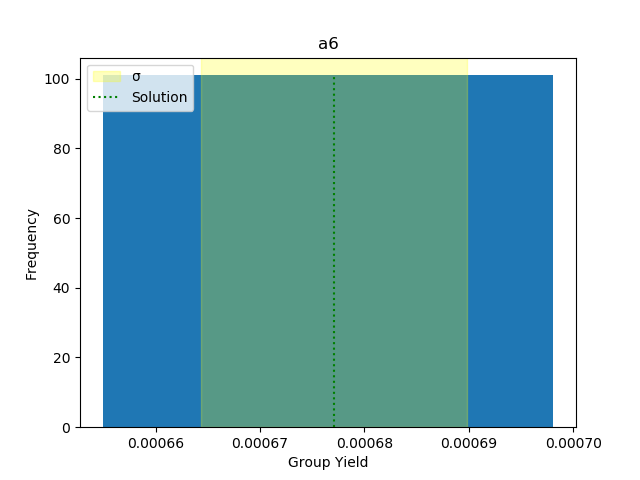
\includegraphics[scale=0.55]{images/ga6-yield-MC.png}
    \caption{5,000 stochastic uncertainty simulations of the Keepin, Wimett, and Zeigler sixth precursor group yield using a $\mu$ value of 0.5\%.}
    %\caption{Keepin, Wimett, and Zeigler six group data fitting at a 0.5\% meshing of half-lives from a start of 5\% with three possible half-lives per group and using 5,000 stochastic uncertainty runs.}
    \label{fig:a6-uncert}
\end{figure}

%The terms with uncertainties include the decay constants based on the meshing, the number of fission events in the sample, the IAEA decay constants, the IAEA emission probabilities, and the ORIGEN concentrations.




Following the group parameter generation is the point reactor kinetics uncertainties that use the forward Euler method. The decay constant uncertainty comes from the group parameter generation; the initial uncertainties in both the number of neutrons at the current time, $\Delta n^{(m)}$, and the number of precursors in the $i^{th}$ group, $\Delta C_g^{(m)}$, are zero; and the group and total delayed neutron fraction uncertainties, $\Delta \beta_{i}$ and $\Delta \beta$, respectively, are given in Equations \eqref{eq:betai} and \eqref{eq:beta}:


\begin{equation}
\Delta \beta_{i} = \sqrt{ \left(\frac{1}{\bar{\nu}} \Delta\bar{\nu}_{d, g} \right)^2 +
\left( \frac{\bar{\nu}_{d, g}}{\bar{\nu}^2} \Delta \bar{\nu} \right)^2}
\label{eq:betai},
\end{equation}

\begin{equation}
\Delta \beta = \sqrt{ \left(\sum_{i=1}^{n} \Delta \beta_g^2 \right)}
\label{eq:beta}.
\end{equation}

%Because forward Euler is used, the time step, $\Delta t$, also plays a role in the uncertainty. 
The uncertainty in $n^{(m)}$ from Equation \eqref{eq:n-prk}, rewritten with the fully expanded derivative in Equation \eqref{eq:explicitncur}, is given in Equation \eqref{eq:n-uncert}, with the components given in Equations \eqref{eq:n-conti}--\eqref{eq:n-contf}. In these equations, $\Delta t$ is the time step used in the forward Euler method:

\begin{equation}
\begin{split}
n^{(m)} & =  n^{(m-1)} + \frac{\rho - \beta}{\Lambda} n^{(m-1)} \Delta t \\
& + \sum_{i=1}^n \left( \lambda_g C_g^{(m-1)} \Delta t + \frac{\beta_g}{\Lambda} n^{(m-1)} \lambda_g \Delta t^2- \lambda_g^2 C_g^{(m-1)} \Delta t^2 \right),\\
\label{eq:explicitncur}
\end{split}
\end{equation}
where the partial derivatives are taken with respect to the previous time step's number of neutrons, $n^{(m-1)}$; decay constant for each group, $\lambda_g$; delayed neutron fraction, $\beta$; delayed neutron fraction for each group, $\beta_g$; and the previous time step's precursor concentration for each group, $C_g^{(m-1)}$.
The partial derivatives are given as:
\begin{equation}
\frac{\partial n^{(m)}}{\partial n^{(m-1)}} = 1 + \frac{\rho - \beta}{\Lambda} \Delta t + \sum_{i=1}^{n} \frac{\beta_g}{\Lambda} \lambda_g \Delta t^2
\label{eq:n-conti},
\end{equation}
\begin{equation}
\frac{\partial n^{(m)}}{\partial \lambda_g} = C_g^{(m-1)} \Delta t + \frac{\beta_g}{\Lambda} n^{(m-1)} \Delta t^2 - 2 \lambda_g C_g^{(m-1)} \Delta t^2,
\end{equation}
\begin{equation}
\frac{\partial n^{(m)}}{\partial \beta} = \frac{-n^{(m-1)} \Delta t}{\Lambda},
\end{equation}
\begin{equation}
\frac{\partial n^{(m)}}{\partial \beta_g} = \frac{n^{(m-1)} \lambda_g \Delta t^2}{\Lambda},
\end{equation}
\begin{equation}
\frac{\partial n^{(m)}}{\partial C_g^{(m-1)}} = \lambda_g \Delta t - \lambda_g^2 \Delta t^2
\label{eq:n-contf}.
\end{equation}
The partial derivatives are then used to calculate the uncertainty in the number of neutrons at iteration $m$:
\begin{equation}
\begin{split}
\left( \Delta n^{(m)} \right) ^2= & \sum_{i=1}^n\left( \frac{\partial n(t)}{\partial n^{(m-1)}} \Delta n^{(m-1)} \right)^2 + \left( \frac{\partial n(t)}{\partial \lambda_g} \Delta \lambda_g \right)^2 \\
 & + \left( \frac{\partial n(t)}{\partial \beta} \Delta \beta \right)^2 + \left( \frac{\partial n(t)}{\partial \beta_g} \Delta \beta_g \right)^2 \\
 & + \left( \frac{\partial n(t)}{\partial C_g^{(m-1)}} \Delta C_g^{(m-1)} \right)^2.
\end{split}
\label{eq:n-uncert}
\end{equation}

The uncertainty in $C_g$ from \eqref{eq:c-prk}, rewritten with the fully expanded derivative in Equation \eqref{eq:explciitC}, is given by Equation \eqref{eq:C-uncert}, incorporating the components given by Equations \eqref{eq:C-conti}--\eqref{eq:C-contf}:
\begin{equation}
C_g^{(m)} = C_g^{(m-1)} + \frac{\beta_g}{\Lambda} n^{(m-1)} \Delta t - \lambda_g \Delta t C_g^{(m-1)},
\label{eq:explciitC}
\end{equation}
where the partial derivatives are taken with respect to the same variables as the equation for the number of neutrons:
\begin{equation}
\frac{\partial C_g^{(m)}(t)}{\partial C_g^{(m-1)}} = 1 - \lambda_g \Delta t
\label{eq:C-conti},
\end{equation}
\begin{equation}
\frac{\partial C_g^{(m)}}{\partial \beta_g} = \frac{n^{(m-1)} \Delta t}{\Lambda},
\end{equation}
\begin{equation}
\frac{\partial C_g^{(m)}}{\partial n^{(m-1)}} = \frac{\beta_g \Delta t}{\Lambda},
\end{equation}
\begin{equation}
\frac{\partial C_g^{(m)}}{\partial \lambda_g} = - C_g^{(m-1)} \Delta t
\label{eq:C-contf}.
\end{equation}

The partial derivatives are then used to calculate the uncertainty in each precursor group concentration at iteration $m$:
\begin{equation}
\begin{split}
\left( \Delta C_g^{(m)} \right)^2 = & \sum_{i=1}^n\left( \frac{\partial C_g^{(m)}}{\partial n^{(m-1)}} \Delta n^{(m-1)} \right)^2 + \left( \frac{\partial C_g^{(m)}}{\partial \lambda_g} \Delta \lambda_g \right)^2 \\
& + \left( \frac{\partial C_g^{(m)}}{\partial \beta_g} \Delta \beta_g \right)^2 + \left( \frac{\partial C_g^{(m)}}{\partial C_g^{(m-1)}} \Delta C_g^{(m-1)} \right)^2 .
\label{eq:C-uncert}
\end{split}
\end{equation}

Finally, the uncertainty of group spectra constructed using the iterative linear least squares procedure is shown in Equation \eqref{eq:spec-base}.
This uncertainty is fairly straightforward to calculate because the delayed neutron count term, $\dot{n}_d(t)$, comes from the six group parameters for which the uncertainty is given in Equation \eqref{eq:delnu-uncert}.
The uncertainty for the energy-dependent neutron emission count rate is shown in Equation \eqref{eq:spec-uncert}, where the uncertainty in the spectra, $\Delta \chi_g(E)$, is calculated stochastically, in the same manner as the group yield uncertainties:
\begin{equation}
\dot{n}_d(E, t) = \dot{n}_d(t) \sum_g \chi_g (E)
\label{eq:spec-base},
\end{equation}
\begin{equation}
\Delta n_d^2(E, t) = \left( \Delta \dot{n}_d(t) \sum_g \chi_g(E) \right)^2 + \left( \left( \dot{n}_d(t) \right)^2 \sum_g \left( \Delta \chi_g(E) \right)^2 \right) \hspace{-2pt} .
\label{eq:spec-uncert}
\end{equation}




%%%%%%%%%%%%%%%%%%%%%%%%%%%%%%%%%%%%%%%%%%%%%%%%%%%%%%%%%%%%%%%%%%%%%%%%%%%%%%%%
\section{Results and Analysis}


%%%%%%%%%%%%%%%%%%%%%%%%%%%%%%%%%%%%%%%%%%%%%%%%%%%%%%%%%%%%%%%%%%%%%%%%%%%%%%%%
\subsection{ORIGEN Data Compared with IAEA Data}

Because the group parameters are fit to the delayed neutron count data, it is important to understand how the data compare.
The two different datasets compared are the previously discussed IAEA--ORIGEN and the Pure ORIGEN datasets.
%The end7dec library is referred to as \textit{Pure ORIGEN}, and it uses modified ENDF/B-VII.0 data with an embedded version of SOURCES4C.
For analysis of delayed neutron emission count rate, the three components that can change from the datasets are the time-dependent compositions term, the decay constants term, and the emission probabilities term, all of which were first presented in Equation \eqref{eq:ndiaea}.

The composition as a function of time depends on the incident fission neutron energy, the fission yield, the decay constant of the target isotope, and that same data for any isotopes that decay into the target isotope. In this work, the ORIGEN- and IAEA-based data comparisons use the compositions generated by KENO-VI and decayed in ORIGEN.

%The decay constants, $\lambda$, and emission probabilities (or branching fractions), $P_n$, can be tested by comparing the results of the Pure ORIGEN dataset simulated in ORIGEN with the IAEA dataset in ORIGEN.
We can conduct a sensitivity study of the decay constants, $\lambda$, and emission probabilities (or branching fractions), $P_n$, by comparing the results of the Pure ORIGEN dataset simulated in ORIGEN with the IAEA dataset in ORIGEN.
Specifically, we can adjust the data such that only decay constants, only emission probabilities, or both are swapped from the Pure ORIGEN dataset values to the IAEA dataset values.

%\begin{figure}[]
%\centering
%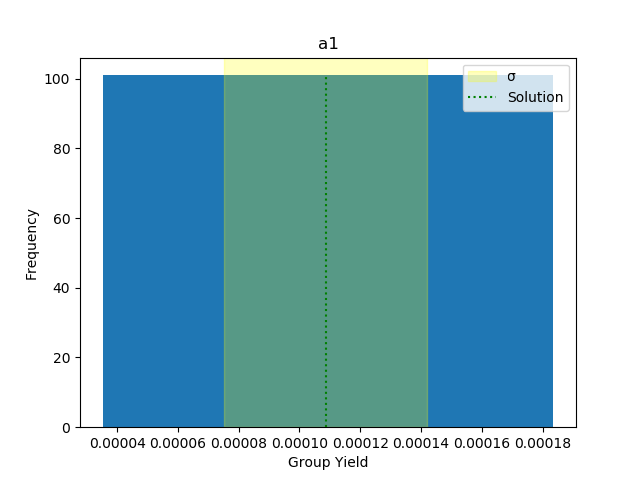
\includegraphics[width=0.23\textwidth]{images/PURE-IAEA-COMP/ga1-yield-MC.png}
%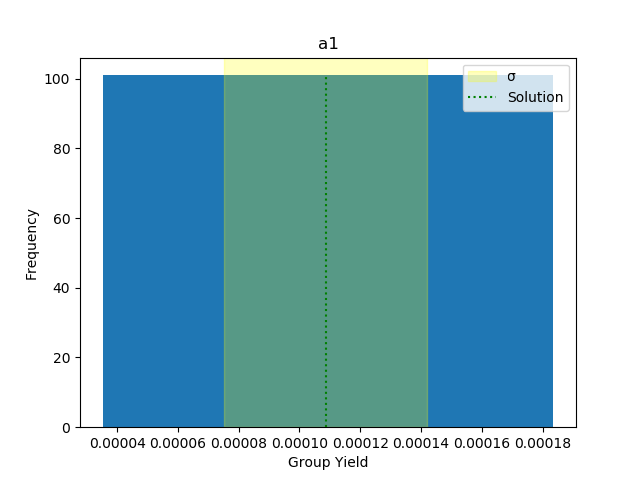
\includegraphics[width=0.23\textwidth]{images/PURE-IAEA-COMP/ga1-yield-MC.png}
%\caption{Plot of delayed neutron count rate with IAEA and Pure ORIGEN decay constants (top). Plot of isotopes' contribution to difference between %count rates (bottom).}
%\end{figure}

%\begin{figure}[]
%\centering
%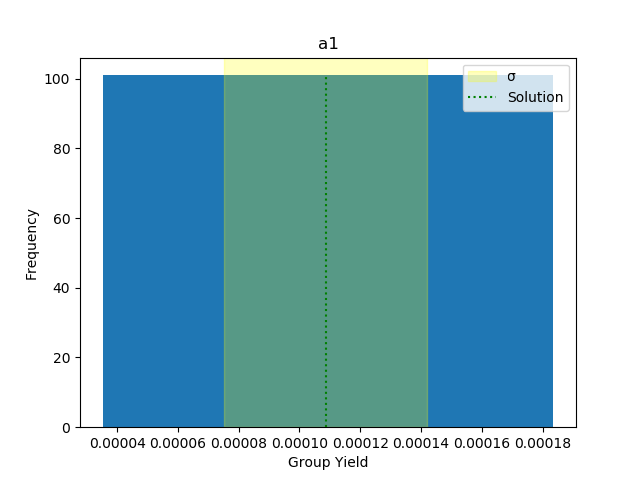
\includegraphics[width=0.23\textwidth]{images/PURE-IAEA-COMP/ga1-yield-MC.png}
%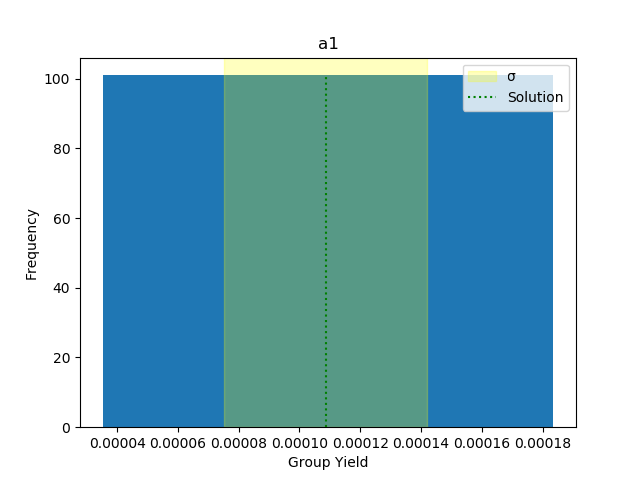
\includegraphics[width=0.23\textwidth]{images/PURE-IAEA-COMP/ga1-yield-MC.png}
%\caption{Plot of delayed neutron count rate with IAEA and Pure ORIGEN emission probabilities (top). Plot of isotopes' contribution to difference %between count rates (bottom).}
%\end{figure}

%\begin{figure}[]
%\centering
%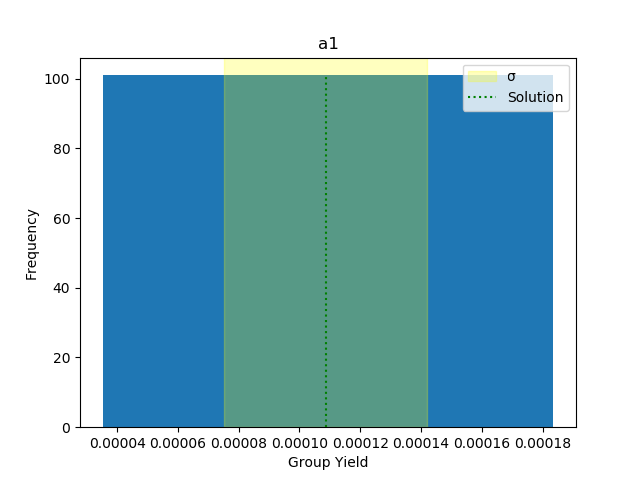
\includegraphics[width=0.23\textwidth]{images/PURE-IAEA-COMP/ga1-yield-MC.png}
%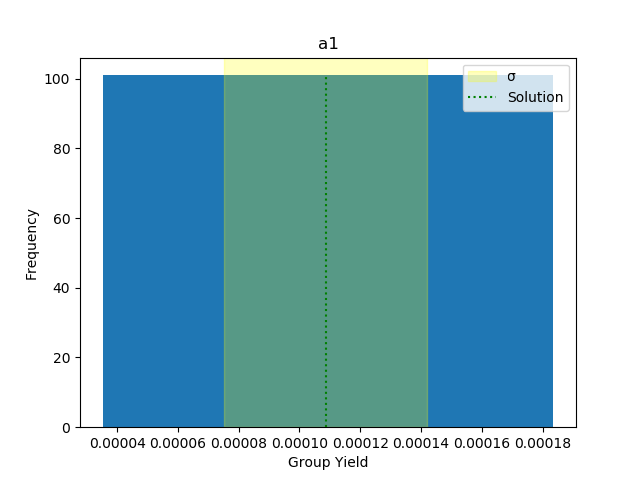
\includegraphics[width=0.23\textwidth]{images/PURE-IAEA-COMP/ga1-yield-MC.png}
%\caption{Plot of delayed neutron count rate with IAEA and Pure ORIGEN decay constants and emission probabilities (top). Plot of isotopes' %contribution to difference between count rates (bottom).}
%\end{figure}

%\begin{figure}[]
%\centering
%\includegraphics[width=0.45\textwidth]{images/PURE-IAEA-COMP/total-compare.png}
%\includegraphics[width=0.45\textwidth]{images/PURE-IAEA-COMP/perc_diff-full-pcnt.png}
%\caption{Plot of Pure ORIGEN counts (top) and IAEA--ORIGEN counts as well as the percent difference between the two (bottom).}
%\label{fig:count-diff}
%\end{figure}

\begin{figure}[]
\def\tabularxcolumn#1{m{#1}}
\begin{tabularx}{\linewidth}{@{}cXX@{}}
%
\begin{tabular}{cc}
\subfloat[Pure ORIGEN and IAEA--ORIGEN count rate over time]{\includegraphics[width=0.45\linewidth]{images/total-compare.png}} &
\subfloat[Pure ORIGEN and IAEA--ORIGEN count rate difference over time normalized by the IAEA--ORIGEN count rate]{\includegraphics[width=0.45\linewidth]{images/perc_diff-full-pcnt.png}}\\
\end{tabular}
\end{tabularx}

\caption{Comparison of delayed neutron count rate for Pure ORIGEN and IAEA--ORIGEN data after fast-pulse irradiation of \ce{^{235}U}.}\label{fig:count-diff}
\end{figure}

Figure \ref{fig:count-diff} shows the net count rate for the Pure ORIGEN and for the IAEA--ORIGEN data sets in which the percent difference of the Pure ORIGEN to the IAEA--ORIGEN count rate appears to be close. The percent difference between the count rates initially starts at $\sim$1.5\%, peaks at a 14\% difference shortly thereafter, and then drops again. %From the shape of the percent difference, it appears that short-lived isotopes decay away and reduce the difference.
Figures \ref{fig:start-comp}--\ref{fig:end-comp} provide more information on the short-lived and longer-lived isotopes that lead to this percent difference. 
These figures are generated by comparing count rate differences from decay constants, emission probabilities, and both at the same time.
The plots show the difference of the Pure ORIGEN count rate with the IAEA--ORIGEN count rate subtracted away.
The negative count rate differences are represented as dashed lines, while the positive count rate differences are solid lines.
The nuclides are selected by tracking whichever nuclides have the largest absolute difference at each time step, as the shorter lived nuclides will have a smaller absolute difference as they decay away.
Figure \ref{fig:start-comp} shows that the peak decay constant difference causes around 1.2 million counts per second, while the difference drops rapidly during later times. 
The count rate difference is larger because of the emission probability difference than the decay constant difference.
This can be seen by comparing the differences in Figures \ref{fig:start-comp} and \ref{fig:emis-prob} at various times.
%The emission probabilities have a smaller maximum effect, but the integral effect is larger; therefore, the combined effects of emission and decay constants are dominated by precursors that are significantly affected by emission probability data differences.
%\begin{figure}[]
%\centering
%\includegraphics[width=0.45\textwidth]{images/PURE-IAEA-COMP/origen_iaea_dn_targets-pre10-lam.png}
%\includegraphics[width=0.45\textwidth]{images/PURE-IAEA-COMP/origen_iaea_dn_targets-post10-lam.png}
%\caption{Decay constant--based difference between count rates with IAEA decay constants for \ce{^{235}U} fast-pulse irradiation over different time frames.}
%\label{fig:start-comp}
%\end{figure}

\begin{figure}[]
\centering
\includegraphics[width=0.48\textwidth]{images/origen_ensdf_dn_targets_lam.png}
\caption{The decay constant--based difference between Pure ORIGEN count rates and Pure ORIGEN with IAEA decay constants for \ce{^{235}U} fast-pulse irradiation over time. The dotted lines represent a negative count rate difference, meaning the IAEA decay constants increase the count rate for those nuclides.}
\label{fig:start-comp}
\end{figure}

%\begin{figure}[]
%\def\tabularxcolumn#1{m{#1}}
%\begin{tabularx}{\linewidth}{@{}cXX@{}}
%%
%\begin{tabular}{cc}
%\subfloat[Short time scale]{\includegraphics[width=0.45\linewidth]{images/PURE-IAEA-COMP/origen_iaea_dn_targets-%pre10-lam.png}} & 
%\subfloat[Long time scale]{\includegraphics[width=0.45\linewidth]{images/PURE-IAEA-COMP/origen_iaea_dn_targets-%post10-lam.png}}\\
%\end{tabular}
%\end{tabularx}
%
%\caption{Decay constant--based difference between count rates with IAEA decay constants for \ce{^{235}U} fast-%pulse irradiation over different time frames.}
%\label{fig:start-comp}
%\end{figure}

%\begin{figure}[]
%\centering
%\includegraphics[width=0.45\textwidth]{images/PURE-IAEA-COMP/origen_iaea_dn_targets-pre50-pn.png}
%\includegraphics[width=0.45\textwidth]{images/PURE-IAEA-COMP/origen_iaea_dn_targets-post50-pn.png}
%\caption{Emission probability (i.e., branching fraction)--based difference between count rates with IAEA decay constants for \ce{^{235}U} fast-pulse irradiation over different time frames.}
%\label{fig:emis-prob}
%\end{figure}

\begin{figure}[]
\centering
\includegraphics[width=0.48\textwidth]{images/origen_origen_dn_targets_pn.png}
\caption{The emission probability (i.e., branching fraction)--based difference between the Pure ORIGEN count rates and Pure ORIGEN with IAEA decay constants for \ce{^{235}U} fast-pulse irradiation over time. The dotted lines represent a negative count rate difference, meaning the IAEA emission probabilities increase the count rate for those nuclides.}
\label{fig:emis-prob}
\end{figure}

%\begin{figure}[]
%\def\tabularxcolumn#1{m{#1}}
%\begin{tabularx}{\linewidth}{@{}cXX@{}}
%%
%\begin{tabular}{cc}
%\subfloat[Short time scale]{\includegraphics[width=0.45\linewidth]{images/PURE-IAEA-COMP/origen_iaea_dn_targets-%pre50-pn.png}} & 
%\subfloat[Long time scale]{\includegraphics[width=0.45\linewidth]{images/PURE-IAEA-COMP/origen_iaea_dn_targets-%post50-pn.png}}\\
%\end{tabular}
%\end{tabularx}
%
%\caption{Emission probability (i.e., branching fraction)--based difference between count rates with IAEA decay %constants for \ce{^{235}U} fast-pulse irradiation over different time frames.}
%\label{fig:emis-prob}
%\end{figure}

%\begin{figure}[]
%\centering
%\includegraphics[width=0.45\textwidth]{images/PURE-IAEA-COMP/origen_iaea_dn_targets-pre50-net.png}
%\includegraphics[width=0.45\textwidth]{images/PURE-IAEA-COMP/origen_iaea_dn_targets-post50-net.png}
%\caption{Combined decay constant and emission probability--based difference between count rates with IAEA decay constants for \ce{^{235}U} fast-pulse irradiation over different time frames.}
%\label{fig:end-comp}
%\end{figure}

\begin{figure}[]
\centering
\includegraphics[width=0.48\textwidth]{images/origen_iaea_dn_targets_net.png}
\caption{The combined decay constant and emission probability--based difference between Pure ORIGEN count rates and IAEA--ORIGEN count rates for \ce{^{235}U} fast-pulse irradiation over time. The dotted lines represent a negative count rate difference, meaning the combined IAEA decay constants and emission probabilities increase the count rate for those nuclides.}
\label{fig:end-comp}
\end{figure}



%\begin{figure}[]
%\def\tabularxcolumn#1{m{#1}}
%\begin{tabularx}{\linewidth}{@{}cXX@{}}
%%
%\begin{tabular}{cc}
%\subfloat[Short time scale]{\includegraphics[width=0.45\linewidth]{images/PURE-IAEA-COMP/origen_iaea_dn_targets-%pre50-net.png}} &
%\subfloat[Long time scale]{\includegraphics[width=0.45\linewidth]{images/PURE-IAEA-COMP/origen_iaea_dn_targets-%post50-net.png}}\\
%\end{tabular}
%\end{tabularx}
%
%\caption{Combined decay constant and emission probability--based difference between count rates with IAEA decay %constants for \ce{^{235}U} fast-pulse irradiation over different time frames.}
%\label{fig:end-comp}
%\end{figure}





\begin{table}[]
\centering
\caption{Decay and Emission data for isotopes with the largest count rate discrepancies.}
\begin{tabular}{|l l l l l l l|} 
 \hline
 Isotope & $\lambda_{IAEA} \; [s^{-1}]$ & $\lambda_{ORIGEN} \; [s^{-1}]$ & $\Delta \lambda \; [s^{-1}]$ & $P_{IAEA}$ & $P_{ORIGEN}$ & $\Delta P$\\
 \hline\hline
     $^{91}$Br & 1.27 & 1.28 & 0.01 & 0.304 & 0.109 & 0.195\\
     $^{85}$As & 0.343 & 0.343 & 0.00 &  0.625 & 0.22 & 0.405\\
     $^{86}$As & 0.734 & 0.733 & 0.001& 0.345 & 0.105 & 0.240\\
     $^{137}$I & 0.028 & 0.028 & 0.00 & 0.076 & 0.072 & 0.004 \\
     $^{138}$I & 0.111 & 0.111 & 0.00 & 0.053 & 0.026 & 0.027 \\
     $^{86}$Ge & 3.12 & 7.30 & 4.18 & 0.45 & 0.22 & 0.23\\
     $^{98m}$Y & 0.299 & 0.347 & 0.048 & 0.034 & 0.034 & 0.00\\
     $^{140}$I & 1.17 & 0.806 & 0.364 & 0.079 & 0.22 & 0.141\\
     $^{97}$Y & 0.185 & 0.185 & 0.00 & 5.8E-4 & 0.003 & 0.00242\\
 \hline
\end{tabular}
\label{table:worst-isos}
\end{table}

Table \ref{table:worst-isos} lists the isotopes that have the most significant effect on the decay constant and emission probability data differences.
Figures \ref{fig:emis-prob} and \ref{fig:end-comp} show the impact these nuclides have on the delayed neutron count rate. 
%Based on Table \ref{table:worst-isos}, it can be seen that the main difference in the delayed neutron count rates is caused by emission probabilities.
From Table \ref{table:worst-isos}, it can be seen that the emission probabilities affect the majority of the nuclides with the largest differences.
These emission probability differences drive differences in the net yield as well.
Table \ref{table:datasets} shows the net yields from various data sets, and shows that changing the decay constants does not largely impact the net yield.
However, changing emission probabilities has a non-negligible impact of approximately 200 pcm.
This is because the net yield measures the total number of delayed neutrons, which means the time at which they are emitted is less important than the net number that are emitted.



\begin{figure}[]
\centering
\includegraphics[width=0.48\textwidth]{images/0.png}
\caption{Normalized difference in emission spectra of Pure ORIGEN and IAEA--ORIGEN for \ce{^{235}U} fast-pulse irradiation at 0~s with uncertainty tracked for the IAEA-ORIGEN results.}
\label{fig:net-spec}
\end{figure}

Figure \ref{fig:net-spec} shows how the initial spectrum of the ORIGEN output compares to the IAEA--ORIGEN spectrum, with uncertainties, immediately after irradiation.
Although these results account for only one time step, the spectral differences become smaller over time, as shown in Figure \ref{fig:spec-diff}.
While Figure \ref{fig:net-spec} shows the energy spectra at a single time step, Figure \ref{fig:spec-diff} shows the difference of the average of the energy spectra at each time step.
Figure \ref{fig:spec-diff} shows that the IAEA--ORIGEN yields a larger average energy than the Pure ORIGEN data at every time step, which is demonstrated in Figure \ref{fig:net-spec}.
This discrepancy between the energy spectra shortly after irradiation aligns with the previously discussed results.
%The IAEA--ORIGEN data account for 92\% of the spectra when weighing by net yield and the individual isotope contribution to the yield.
Additionally, because the main differences occur in the first 2~s, the problematic isotopes can be determined directly. The results shown in Figures \ref{fig:start-comp}--\ref{fig:end-comp} indicate that those isotopes that differ most significantly within the first 2~s are $^{91}$Br, $^{85}$As, $^{86}$As, $^{137}$I, and $^{138}$I.

\begin{figure}[]
\centering
\includegraphics[width=0.48\textwidth]{images/l2normdiff.png}
\caption{Difference in average delayed neutron energy of Pure ORIGEN and IAEA--ORIGEN for \ce{^{235}U} fast-pulse irradiation over time where Pure ORIGEN is subtracted from IAEA--ORIGEN.}
\label{fig:spec-diff}
\end{figure}
%%%%%%%%%%%%%%%%%%%%%%%%%%%%%%%%%%%%%%%%%%%%%%%%%%%%%%%%%%%%%%%%%%%%%%%%%%%%%%%%
\subsection{Six Group Parameters}
\label{sec:sixgroupfit}

The DNP six groups can be calculated using the generated delayed neutron count rate data and iterative least squares method.
Recall from Section \ref{sec:methods} that a detector efficiency, $\epsilon$, of 3.75E-8 is used in all results to reflect the experimental results from Keepin, Wimett, and Zeigler \cite{KEEPIN1957IN2}.

\begin{table}[]
%\caption{Yields below the line are from studies conducted by Keepin, Wimett, and Zeigler \cite{KEEPIN1957IN2} and by Brady and England \cite{doi:10.13182/NSE103-129}.}
\caption{Net delayed neutron yields from various sources of data for fast $^{235}U$ (partially recreated from \cite{doi:10.13182/NSE103-129, huynh2014calculation}).}
\centering
\begin{tabular}{|l l c|} 
 \hline
 $\lambda$ & $P_n$ & Yield \\
 \hline\hline
     IAEA & IAEA & 0.0191 \\
   ORIGEN & IAEA & 0.0193 \\
   IAEA & ORIGEN & 0.0172 \\
  ORIGEN & ORIGEN & 0.0172 \\
 \hline
  Keepin, Wimett, and Zeigler \cite{KEEPIN1957IN2} & Keepin, Wimett, and Zeigler \cite{KEEPIN1957IN2} & 0.0165 \\
 Brady and England \cite{doi:10.13182/NSE103-129} & Brady and England \cite{doi:10.13182/NSE103-129} & 0.0206 \\
 Tuttle \cite{tuttle1979delayed} & Tuttle \cite{tuttle1979delayed} & 0.0167 \\
 ENDF/B-V \cite{endfb5} & ENDF/B-V \cite{endfb5} & 0.0167 \\
 England et al. \cite{WILSON200271} & England et al. \cite{WILSON200271} & 0.0198 \\
 England and Rider \cite{england1983status} & England and Rider \cite{england1983status} & 0.0206 \\
 ENDF/B-VII.0 \cite{chadwick2006endf} & ENDF/B-VII.0 \cite{chadwick2006endf} & 0.0162 \\
 JEFF-2.2 \cite{JEF2.2_2000} & JEFF-2.2 \cite{JEF2.2_2000} & 0.0191 \\
 JEFF-3.1.1 \cite{santamarina2009jeff} & JEFF-3.1.1 \cite{santamarina2009jeff} & 0.0170 \\
 \hline
\end{tabular}

\label{table:datasets}
\end{table}

Table \ref{table:datasets} lists the net yield variance observed between the IAEA data and ORIGEN library data.
Additionally, net yields from other works are shown for fast \ce{^{235}U} irradiation.
Overall, it can be seen that the calculated yields generally agree with the range of values from the literature.
The upper half of the table shows that there is a large difference between the yields based on the emission probability data.
This is because a shift in the decay constant data minimally affects the net yield.

Tables \ref{table:half-lives} and \ref{table:group-yields} contain the group half-life and yield parameters, which were identified using the iterative least squares approach and the group parameters taken from Brady and England, referenced here since they are the parameters used in ENDF, and from Keepin, Wimett, and Zeigler \cite{doi:10.13182/NSE103-129, KEEPIN1957IN2}.
The results from Keepin, Wimett, and Zeigler are directly compared with this work since their experimental setup is replicated.
The results from Brady and England, which use the microscopic approach, use preliminary data from ENDF/B-VI \cite{england1983status}.
Although the methods are similar to the methods in this work, differences can be expected with the Brady and England results because of the difference in the data used.
The uncertainties for the group parameters are given in Tables \ref{table:half-lives-delta} and \ref{table:group-yields-delta}.
An interesting note is that the IAEA group parameters are all smaller than all the other fits, which means that the delayed neutrons will overall be emitted more rapidly compared to the other fits.

\begin{table}[]
\caption{Six group half-lives given in seconds.}
\centering
\begin{tabular}{|l l l l l l l|} 
 \hline
 Fit & $T_1$ & $T_2$ & $T_3$ & $T_4$ & $T_5$ & $T_6$\\
 \hline\hline
    Brady and England \cite{doi:10.13182/NSE103-129} & 52.1 & 21.2 & 5.74 & 2.29 & 0.816 & 0.243\\
    Keepin, Wimett, and Zeigler \cite{KEEPIN1957IN2} & 54.5 & 21.8 & 6.00 & 2.23 & 0.496 & 0.179 \\
    IAEA--ORIGEN & 49.0 & 19.2 & 3.64 & 1.28 & 0.320 & 0.098 \\
    %IAEA & 48.8 & 19.3 & 3.63 & 1.26 & 0.318 & 0.098 \\
    Pure ORIGEN & 51.3 & 20.7 & 6.04 & 2.19 & 0.505 & 0.115 \\
    %Pure & 53.1 & 21.3 & 5.83 & 2.19 & 0.528 & 0.115 \\
 \hline
\end{tabular}
\label{table:half-lives}
\end{table}

\begin{table}[]
\caption{Six group half-lives' uncertainties given in seconds.}
\centering
\begin{tabular}{|l l l l l l l|} 
 \hline
 Fit & $\Delta T_1$ & $\Delta T_2$ & $\Delta T_3$ & $\Delta T_4$ & $\Delta T_5$ & $\Delta T_6$\\
 \hline\hline
    Keepin, Wimett, and Zeigler \cite{KEEPIN1957IN2} & 0.94 & 0.54 & 0.17 & 0.06 & 0.03 & 0.02\\
    IAEA--ORIGEN & 0.245 & 0.096 & 0.018 & 0.006 & 0.002 & 0.001 \\
    %IAEA & 0.976 & 0.385 & 0.073 & 0.030 & 0.006 & 0.002 \\
    Pure ORIGEN & 0.256 & 0.104 & 0.030 & 0.011 & 0.003 & 0.001 \\
    %Pure & 0.266 & 0.106 & 0.03 & 0.01 & 0.003 & 0.001 \\
 \hline
\end{tabular}
\label{table:half-lives-delta}
\end{table}

\begin{table}[]
\caption{Six group yields in delayed neutrons per fission multiplied by 100.}
\centering
\begin{tabular}{|l l l l l l l|} 
 \hline
 Fit & $\bar{\nu}_{d, 1}$ & $\bar{\nu}_{d, 2}$ & $\bar{\nu}_{d, 3}$ & $\bar{\nu}_{d, 4}$ & $\bar{\nu}_{d, 5}$ & $\bar{\nu}_{d, 6}$\\
 \hline\hline
    Brady and England \cite{doi:10.13182/NSE103-129} & 0.072 & 0.372 & 0.355 & 0.797 & 0.327 & 0.137\\
    Keepin, Wimett, and Zeigler \cite{KEEPIN1957IN2} & 0.063 & 0.351 & 0.310 & 0.672 & 0.211 & 0.043 \\
    IAEA--ORIGEN & 0.083 & 0.350 & 0.670 & 0.566 & 0.187 & 0.054 \\
    %IAEA & 0.083 & 0.348 & 0.674 & 0.560 & 0.182 & 0.052 \\
    Pure ORIGEN & 0.071 & 0.308 & 0.244 & 0.711 & 0.300 & 0.091\\
    %Pure & 0.064 & 0.311 & 0.263 & 0.677 & 0.310 & 0.092\\
 \hline
\end{tabular}
\label{table:group-yields}
\end{table}

\begin{table}[]
\caption{Six group yields' uncertainties in delayed neutrons per fission multiplied by 100.}
\centering
\begin{tabular}{|l l l l l l l|} 
 \hline
 Fit & $\Delta \bar{\nu}_{d, 1}$ & $\Delta \bar{\nu}_{d, 2}$ & $\Delta \bar{\nu}_{d, 3}$ & $\Delta \bar{\nu}_{d, 4}$ & $\Delta \bar{\nu}_{d, 5}$ & $\Delta \bar{\nu}_{d, 6}$\\
 \hline\hline
    Keepin, Wimett, and Zeigler \cite{KEEPIN1957IN2} & 0.005 & 0.011 & 0.028 & 0.023 & 0.015 & 0.005\\
    IAEA--ORIGEN & 0.009 & 0.009 & 0.008 & 0.003 & 0.003 & 0.001 \\
    %IAEA & 0.039 & 0.041 & 0.021 & 0.015 & 0.004 & 0.002 \\
    Pure ORIGEN& 0.014 & 0.018 & 0.012 & 0.007 & 0.002 & 0.001\\
    %Pure & 0.002 & 0.003 & 0.004 & 0.004 & 0.002 & 0.001\\
 \hline
\end{tabular}
\label{table:group-yields-delta}
\end{table}


For the group yields, the IAEA fit showed greater weight on the longer-lived groups, which is noticeable when comparing the longest- and shortest-lived group yields. A comparison of the fits is shown in Figure \ref{fig:keepnorm}; this comparison indicates that the DNP group parameters in the current work are similar to other group parameters. The comparison also reveals discrepancies among the other referenced fits, although all of the fits shown are for the same fissile isotope and fast energy spectrum.

\begin{figure}[]
\centering
\includegraphics[width=0.45\textwidth]{images/keepin-normalized-counts.png}
\caption{A comparison of the different fast fission irradiation DNP six group parameters of \ce{^{235}U} normalized to the Keepin, Wimett, and Zeigler six group count rate with uncertainties \cite{KEEPIN1957IN2}.}
\label{fig:keepnorm}
\end{figure}

The discrepancies could be the result of differences in energy spectra causing fission, uncertainty in the number of fission events, uncertainty in the experimental data collected by Keepin, Wimett, and Zeigler (which were fitted), or uncertainty in the nuclear data used in the codes in this work and in Brady and England's work.

\subsection{Six Group Spectra}

Using the six group parameters generated, as well as the energy-dependent count rate from ORIGEN and the constructed data from the IAEA database, the spectral profiles associated with each group can be generated, as shown in Equation \eqref{eq:speceq}.
\begin{comment}
Figure \ref{fig:old-new-spec} shows a comparison of the fractional fitting method and the iterative least squares method, labeled as data fit, implemented in this work.
The figure shows the probability of a delayed neutron to be emitted in each bin with a width of $2\, keV$.

%Figure \ref{fig:ori-iaea-spec} shows how the group spectra of the Pure ORIGEN fit compares with the IAEA--ORIGEN fit.

\begin{figure}[]
\centering
\includegraphics[width=0.45\textwidth]{images/GROUP-SPECTRA/group6-spectra.png}
\caption{Comparison of fractional fitting least squares method and iterative least squares method for the sixth precursor group for IAEA--ORIGEN in \ce{^{235}U} fast-pulse irradiation.}
\label{fig:old-new-spec}
\end{figure}
\end{comment}
Figure \ref{fig:ori-iaea-data-frac} compares the discrepancy between the historical fractional fitting approach and the proposed  iterative least squares approach.
The iterative least squares provides a visually better fit than that of the fractional fitting method.
This is shown specifically at 330 seconds, where the longest lived groups dominate the spectra.
%This is shown at 330~s, but the results are comparable across the other times as well.

%\begin{figure}[]
%\centering
%\includegraphics[width=0.45\textwidth]{images/GROUP-SPECTRA/330s-frac-oriaea.png}
%\includegraphics[width=0.45\textwidth]{images/GROUP-SPECTRA/330s-iter-oriaea.png}
%\caption{Comparison of normalized IAEA--ORIGEN six group spectra using fractional fitting (top) and iterative least squares (bottom) for \ce{^{235}U} pulse irradiation at 330 seconds.}
%\label{fig:ori-iaea-data-frac}
%\end{figure}

\begin{figure}[]
\def\tabularxcolumn#1{m{#1}}
\begin{tabularx}{\linewidth}{@{}cXX@{}}
%
\begin{tabular}{cc}
\subfloat[Fractional fitting]{\includegraphics[width=0.45\linewidth]{images/330s-frac-oriaea.png}} & 
\subfloat[Iterative least squares]{\includegraphics[width=0.45\linewidth]{images/330s-lstsq-oriaea.png}}\\
\end{tabular}
\end{tabularx}

\caption{Comparison of data with normalized IAEA--ORIGEN six group spectra for \ce{^{235}U} pulse irradiation at 330 seconds.}
\label{fig:ori-iaea-data-frac}
\end{figure}

%Figure \ref{fig:ori-iaea-spec} shows that the group fits for the shortest lived precursor group are different between the Pure ORIGEN and the IAEA--ORIGEN spectra.
%This aligns with the previous results shown, which showed the largest discrepancies occur at short time scales.
%The net spectra, shown in Figure \ref{fig:net-spec}, varies significantly between the ORIGEN decay spectral data and the IAEA-based spectral data.

%\begin{figure}[]
%\centering
%\includegraphics[width=0.45\textwidth]{images/GROUP-SPECTRA/group6-spectra-puori.png}
%\includegraphics[width=0.45\textwidth]{images/GROUP-SPECTRA/group6-spectra-oriaea.png}
%\caption{Comparison of normalized group six Pure ORIGEN six group spectra (top) and IAEA--ORIGEN six group spectra (bottom) for \ce{^{235}U} pulse irradiation using iterative least squares.}
%\label{fig:ori-iaea-spec}
%\end{figure}




\subsection{Point Reactor Kinetics Reactivity Insertion}

To observe the effect of altering the group parameters, the response to a reactivity step insertion can be modeled using point reactor kinetics.
In this problem, we use the following parameters: a neutron generation time of 0.1 $\mu s$, an average number of total neutrons per fission of 2.6, and the DNP group parameters from Section \ref{sec:sixgroupfit}.
Figure \ref{fig:PRK-resp} shows the neutron density response to a reactivity step insertion into a reactor with these parameters.

\begin{figure}[]
\centering
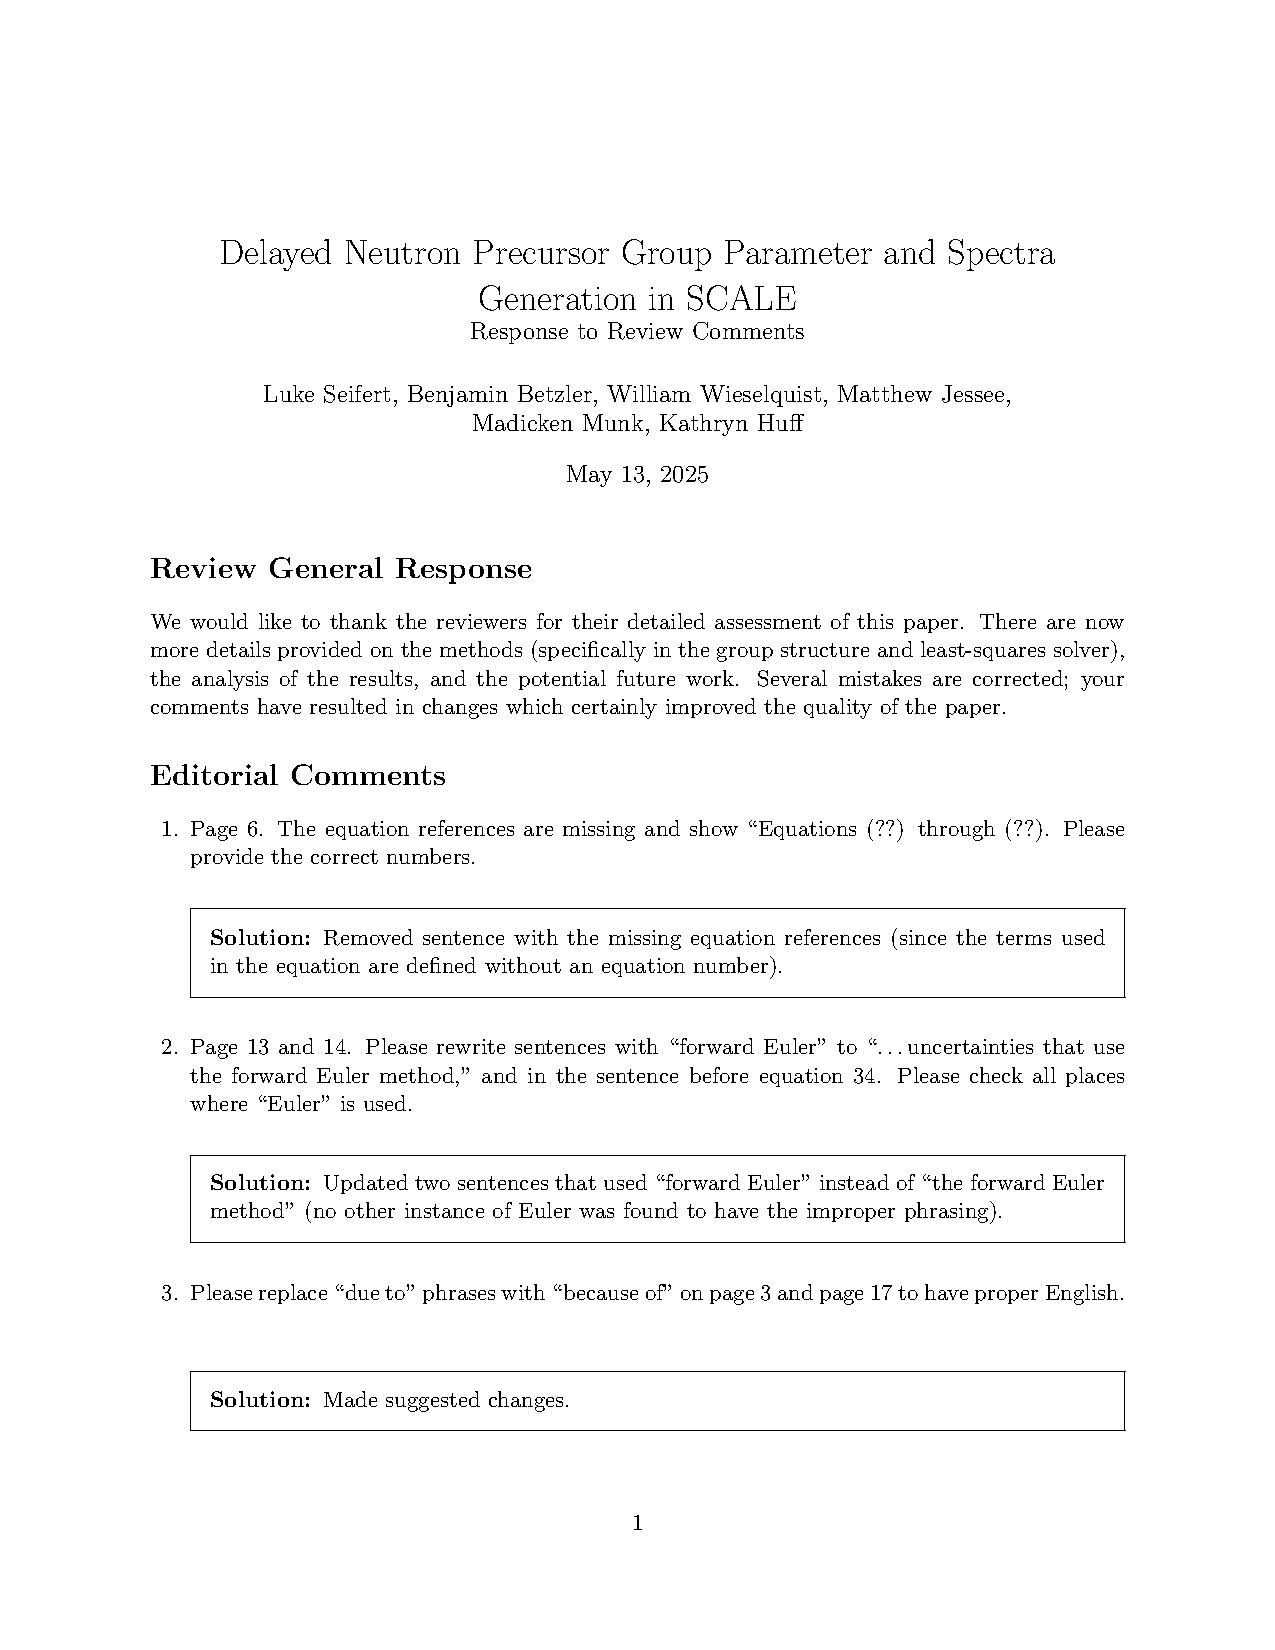
\includegraphics[width=0.45\textwidth]{images/response.png}
\caption{Point reactor kinetic neutron density response to reactivity step insertion for different six group parameters.}
\label{fig:PRK-resp}
\end{figure}

Figure \ref{fig:PRK-resp} shows that the Keepin, Wimett, and Zeigler response was slightly lower than that of the current work \cite{KEEPIN1957IN2}. The responses began closely aligned and diverged further apart as the effect of the DNPs becomes more significant. In the later times, the IAEA--ORIGEN neutron density was slightly lower than the Pure ORIGEN neutron density. This is because the group parameters of Pure ORIGEN have higher yield values for five and six groups, the yield values of which dominate during the early times. This effect was counteracted slightly by the slightly longer lives of five and six groups that Pure ORIGEN also has, but the net effect was still an increased response compared with that of the IAEA--ORIGEN group parameters. Following this logic, the Keepin, Wimett, and Zeigler group parameters have small yields for five and six groups while also having fairly long half- lives for each group.

\subsection{Westinghouse $\mathbf{17\times17}$ Pressurized Water Reactor}
\label{sec:W1717}

Additional macroscopic analysis was conducted using SCALE/Polaris. SCALE/Polaris is a tool used to perform 2D lattice physics that provides six group kinetics parameters as an output. These outputs are importance weighted, nuclide integrated, and assembly homogenized.
Because these kinetics parameters are used by other codes to perform transient analyses, it is important to determine the difference using the default kinetic parameters used as an input compared with the six group parameters generated in this work.

For this analysis, only the fast-spectrum kinetics parameters were altered for \ce{^{235}U}.
This adjustmented was performed to provide a conservative estimate for the magnitude of difference, which can be expected because of the heavily thermal spectrum.

The default values used for the kinetic parameter inputs are those from Keepin, Wimett, and Zeigler \cite{KEEPIN1957IN2}.
The IAEA and Pure ORIGEN six group parameters presented in this work were then used.
The resulting kinetics parameters outputs for each set of group parameters were compared, with the absolute percent differences shown in Figure \ref{fig:Polaris}.

\begin{figure}[]
\centering
\includegraphics[width=0.47\textwidth]{images/group_bar.png}
\caption{The absolute percent difference of IAEA and Pure ORIGEN six group parameters to the Keepin, Wimett, and Zeigler parameters of fast spectrum $^{235}$U in a Westinghouse $17\times17$ fuel assembly.}
\label{fig:Polaris}
\end{figure}

These absolute percent differences from the Keepin, Wimett, and Zeigler data show that the largest difference in IAEA yield and half-life values was observed in the third precursor group; the greatest difference in those values for Pure ORIGEN was observed in the sixth precursor group.
This result corresponds directly to the differences in the six group parameters shown in Tables \ref{table:half-lives} and \ref{table:group-yields}.
In particular, the IAEA-ORIGEN third precursor group has a yield of 0.670, which is almost double the Pure ORIGEN third precursor group yield of 0.244.
Even though fast fission of $^{235}$U in the Westinghouse PWR is not the primary mode of fission, the large difference in the group yield data still leads to a difference of approximately 8\% in the net group 3 yields.

%A brief investigation showed that the largest percent difference from the Keepin, Wimett, and Zeigler fits for both the yields and the half-lives were in the sixth precursor group for the Pure ORIGEN data.
%The same applies for the IAEA data in the third precursor group for the half-lives, but the largest percent difference in half-life was actually in the sixth precursor group.
%However, the third precursor group half-life showed a percent difference over 100\%, whereas the next largest difference was close to 30\%.
%This large difference causes the difference in the third precursor group to dominate over the difference in the sixth precursor group.


%%%%%%%%%%%%%%%%%%%%%%%%%%%%%%%%%%%%%%%%%%%%%%%%%%%%%%%%%%%%%%%%%%%%%%%%%%%%%%%%
\section{Conclusions and Future Work}

This work demonstrates generation of DNP group parameters from a simulated irradiation combined with data from the IAEA and from ORIGEN \cite{DIMITRIOU2021144}.
These group parameters use recent experimental data and propagated uncertainties to investigate the effects on reactor behavior.
The results showed that some of the DNP data used in ORIGEN differs with the data from the IAEA database.

Specifically, a few particular nuclides have large differences between the IAEA database and in ORIGEN.
The nuclides with the largest impact on the delayed neutron count rate following fast spectrum pulse irradiation of $^{235}$U from data discrepancies include $^{91}$Br, $^{85}$As, $^{86}$As, $^{137}$I, $^{138}$I, $^{86}$Ge, $^{98m}$Y, $^{140}$I, and $^{97}$Y.
These discrepancies result in a 200$\,pcm$ difference in the total delayed neutron yield, as well as differences in the rate at which the delayed neutrons are emitted.
The two sets of group parameters generated from this differing data in a point reactor kinetics model showed that the resulting neutron density responses are similar over a relatively short time period after large reactivity insertions.
Discrepancies among the data between SOURCES4C and ENDF are currently being dealt with by relying more on ENDF and less on SOURCES4C where possible in SCALE.

The group spectra generation was also investigated in this work.
The proposed method which allows each DNP to contribute to every DNP group showed promising results, providing a better fit than the fractional fitting method.
The iterative least squares method proposed is more computationally expensive, but it is worthwhile provided the group spectra do not need to be regenerated frequently.

%The point reactor kinetics response provides a useful visualization for the macroscopic effect of updated group fits.
There are many different possible extensions which can further this work.
Updates could be made to the group parameters by implementing updated data and propagating uncertainty.
The group spectra could also be updated with uncertainty propagation and methods for fitting optimal group spectra.
A more thorough analysis of various group parameter fitting methods for yields and spectra could include using non-linear least squares or other least squares methods, calculating uncertainty when the decay constant mesh is refined to the furthest extent possible, and determining whether other methods would alter how many groups are needed for a fit within a given margin.
Analysis of additional data sources, such as the Joint Evaluated Fission and Fusion library, could similarly identify additional isotopes causing discrepancies.
Also of interest are comparisons with kinetics benchmarks by investigating other energy spectra, fissile nuclides, and kinetics methodologies \cite{aboanber2013generalized, ganapol2009refined, nobrega1971new}.
A tool such as Moltres can incorporate these group parameters to simulate 3-dimensional kinetics benchmark problems \cite{lindsay_introduction_2018, park_advancements_2025, kliem1999benchmark, briggs2014overview}.

%%%%%%%%%%%%%%%%%%%%%%%%%%%%%%%%%%%%%%%%%%%%%%%%%%%%%%%%%%%%%%%%%%%%%%%%%%%%%%%%
%\appendix
%\section{Appendix}

%Numbering in the appendix is different:
%\begin{equation} \label{eq:appendix}
%  2 + 2 = 5\,.
%\end{equation}
%and another equation:
%\begin{equation} \label{eq:appendix2}
%  a + b = c\,.
%\end{equation}

%%%%%%%%%%%%%%%%%%%%%%%%%%%%%%%%%%%%%%%%%%%%%%%%%%%%%%%%%%%%%%%%%%%%%%%%%%%%%%%%
\section*{Acknowledgments}
This manuscript has been authored by UT-Battelle, LLC under contract DE-AC05-00OR22725 with the US Department of Energy (DOE). The US government retains and the publisher, by accepting the article for publication, acknowledges that the US government retains a nonexclusive, paid-up, irrevocable, worldwide license to publish or reproduce the published form of this manuscript, or allow others to do so, for US government purposes. DOE will provide public access to these results of federally sponsored research in accordance with the DOE Public Access Plan (http://energy.gov/downloads/doe-public-access-plan).
This material is based upon work supported under an Integrated University Program Graduate Fellowship.
The authors are grateful for this generous support.
Any opinions, findings, conclusions or recommendations expressed in this publication are
those of the author(s) and do not necessarily reflect the views of the Department of Energy
Office of Nuclear Energy.
%Thanks to Friederike Bostelmann and Ugur Mertyurek for their review of this paper.
Thanks to Ugur Mertyurek reviewing this paper.
Additional thanks to the University of Illinois Department of Nuclear, Plasma, and Radiological Engineering and the members of the Advanced Reactors and Fuel Cycles group for their support and suggestions in developing this work.

%\section{Potential Additions}
%\begin{itemize}
%    \item This summary only covers the \ce{^{235}U} pulse irradiation (no infinite, no other fissile isos, etc.)
%    \item Add uncertainties (Currently, this work does not consider the uncertainty in the isotopic spectra provided.) (methods and results)
%    \item Did not include all group spectra, how group spectra match up to actual spectra, how fractional fitting compares for each group.
%    \item Did not include limit when percent variance of decay constant meshing goes to zero for multiple groups.
%    \item Did not include times other than 0s for spectral data.
%    \item Add discussion of pulse vs infinite irradiation
%    \item Include W17x17 results/information
%\end{itemize}


\pagebreak
\bibliographystyle{style/ans_js}                                                                           %custom ANS journal submission template bibliography style
\bibliography{bibliography}

\end{document}


